\newpage
\section{Concise Literature Review}  
\label{S:REVIEW} 

%--------------------------------------------------
\subsubsection{Sea Level}
Sea level plays a unique role in physical oceanography. A role at least partly be attributed to it's \emph{observability}\citep{Wilson:2010hy}.


The present study will be limited to forecasts of sea level over time scales of hours to days; variations that basically constitute `the tides' as far as the general public is concerned.


\begin{figure}[!h]
\begin{center}
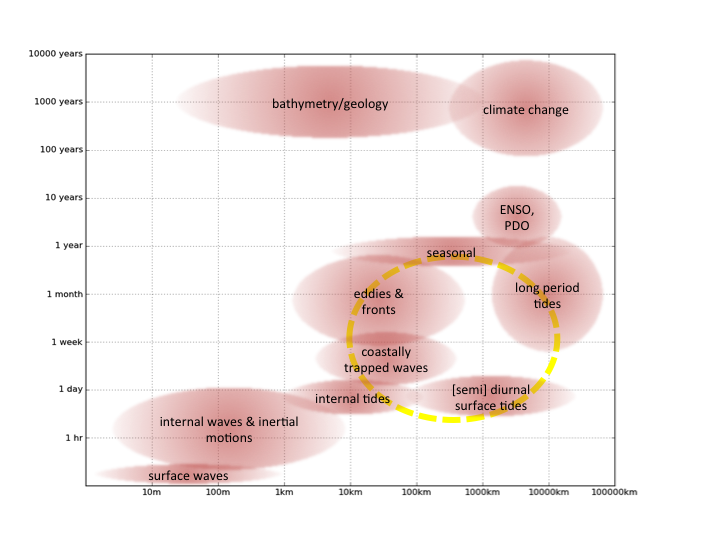
\includegraphics[width=130mm]{figures/images/ocean_scales.png}
\caption{Schematic indication of time/length scales of ocean processes.  The approximate scale limits for this research are highlighted. (Following \citet{Chelton:2001ws} )}
\label{fig:SCALES}
\end{center}
\end{figure}


\begin{figure}[!h]
\begin{center}
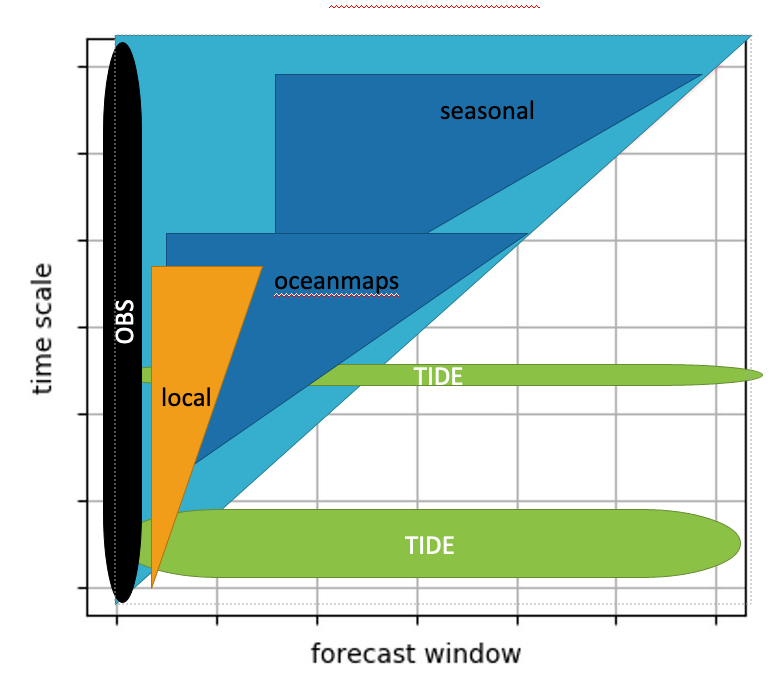
\includegraphics[width=80mm]{figures/images/sealevel_cartoon.png}
\caption{Simplified illustration of the relative nature of sea level and different observing platforms.}
\label{fig:SEALEVEL}
\end{center}
\end{figure}


\begin{figure}[!h]
	\centering
	\subfloat[Darwin in Northern Australia - large diurnal tide.]{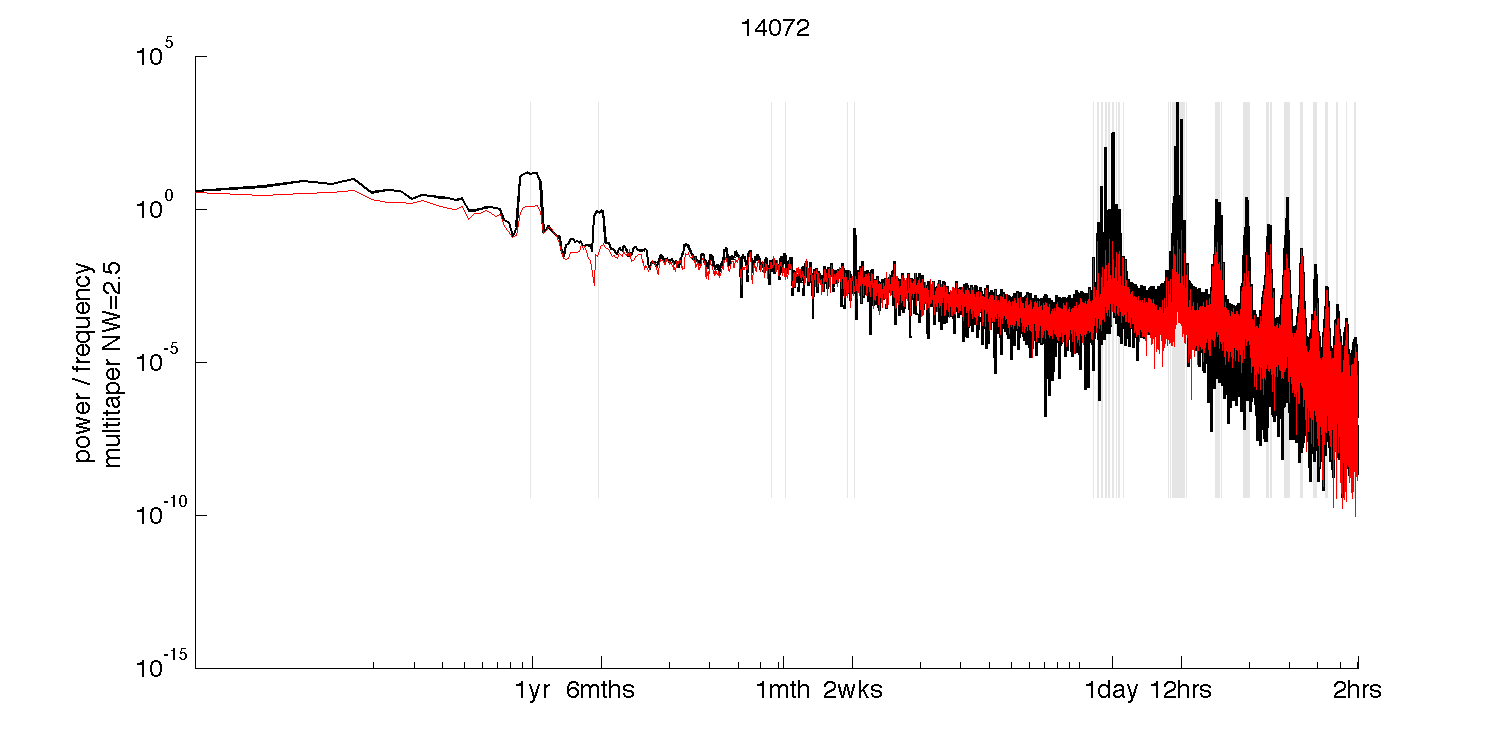
\includegraphics[width=130mm]{figures/images/plot_14072.png}} \\
	\subfloat[Esperence in Southern Australia - powerful synoptic signal.]{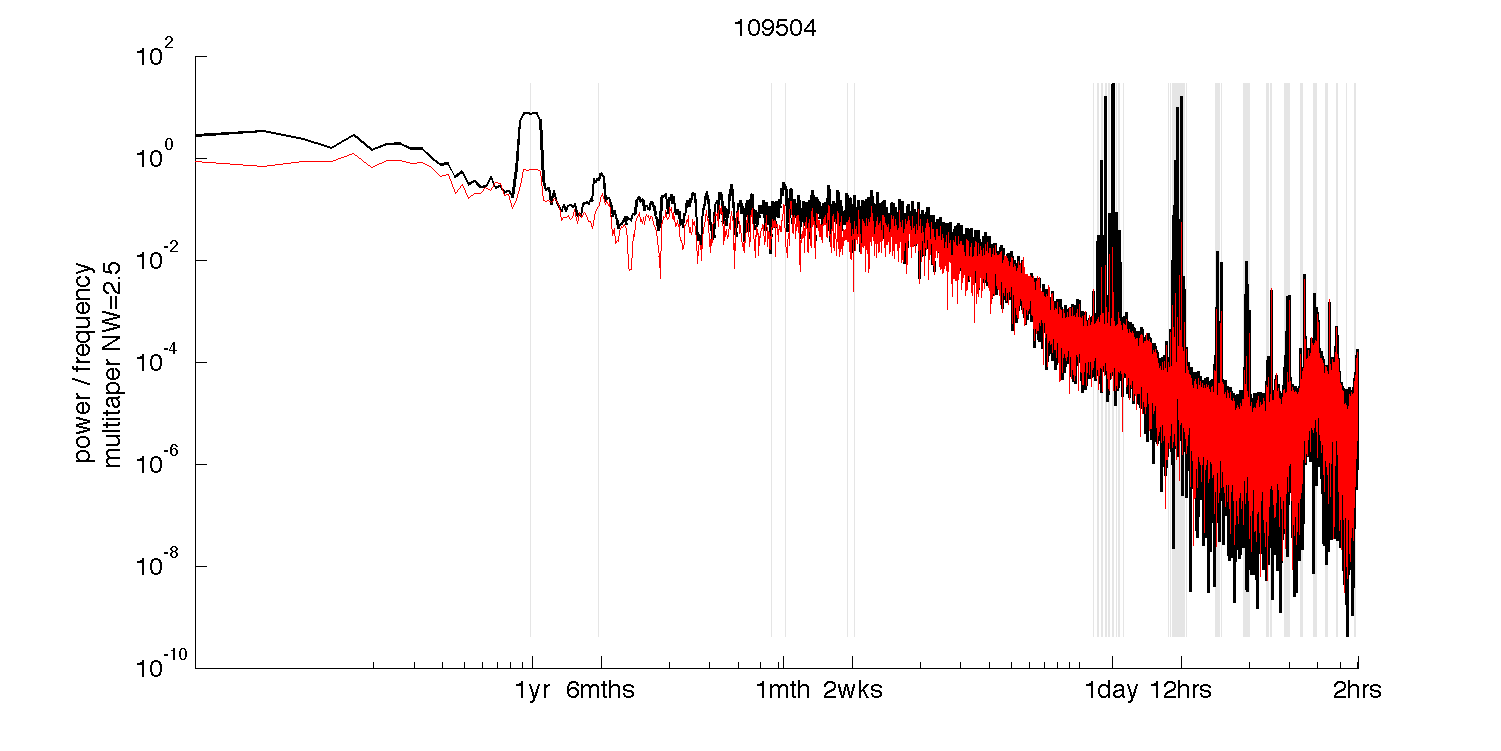
\includegraphics[width=130mm]{figures/images/plot_109504.png}}
	\caption{Spectral estimates from two coastal tide gauges. Hourly data, black = observations, red = tidal residual. An example of a `mixed spectra' \citep{Percival:1998tw}, in the sense of that discrete spectral lines appear embedded in a background continuum of coloured noise.  The overall `redness' of the spectra and the prominence of spikes at tidal frequencies is highlighted }
    \label{fig:SPECTRA_EG}
\end{figure}


%--------------------------------------------------
\subsubsection{Literature and Operations}
\label{S:operational_setting}

Operational considerations are relevant to this review, which does not launch neatly from a single `conversation' \citep{Booth:2009vy} in the scientific literature.\\
Unfortunately operational documentation often falls far behind aspirations.
Tidal observation manuals exist eg \citep{IOC:2005tj}, \citep{Level:2011wu}, \citep{Parker:2007wq}.  However, analysis methods and design justifications are less formally documented - if at all.  The IOC understates this situation simply: `many organizations have developed their own method of tidal analysis'\citep{IOC:2005tj}\\

User expectations of sea level forecasts have largely been defined by harmonic tidal prediction practice. 
Conversely operational practice have influenced oceanography more broadly. Doodson's \citep{Doodson:1928wf} tidal procedures reflect the practical limits imposed by human computers and paper records, but have ongoing influence. \\

%-------------------------------------------------- 
\subsubsection{Intersection of Two Perspectives}
\label{S:two_perspectives}

Tidal harmonic methods have for many decades provided the only routine source of sea level forecast - and with great success.  
In contrast, time stepping primitive equation dynamic models and data assimilation are relatively new arrivals to operational centres.  
These represent two qualitatively different perspectives on sea level prediction.\\



Over the past decade, the operational evolution of \OGCM-based prediction has increasingly brought the two approaches into something akin to Gallison's `trading zone' \citep{Galison:1996uc}.
Developments promise only to increase the amount of overlap into the previously independent practices of harmonic analysis, eg \cite{Arbic:2010us}.\\
Here Munk and Cartwright's aphorism from the 1960's regarding tidal analysis is illustrative:
\begin{quote}
\dots predicting and learning are in a sense orthogonal, and the most interesting effects are those that cause the most trouble with a forecasting: the continuum, the nongravitational tides, and the non-linear interactions.\citep{Munk:1966ts} 
\end{quote}
Forecasts from \BL{} and other similar systems now represent sea level attributable to exactly these troublesome areas; or at least some physical subset therein.
Jayne's reference to the ``vexing problems'' \citep[pp812]{Jayne:2001tr} arising from applying frequency-domain theory in time-domain numerical tide modelling is illustrative.


\begin{figure}[h]
\begin{center}
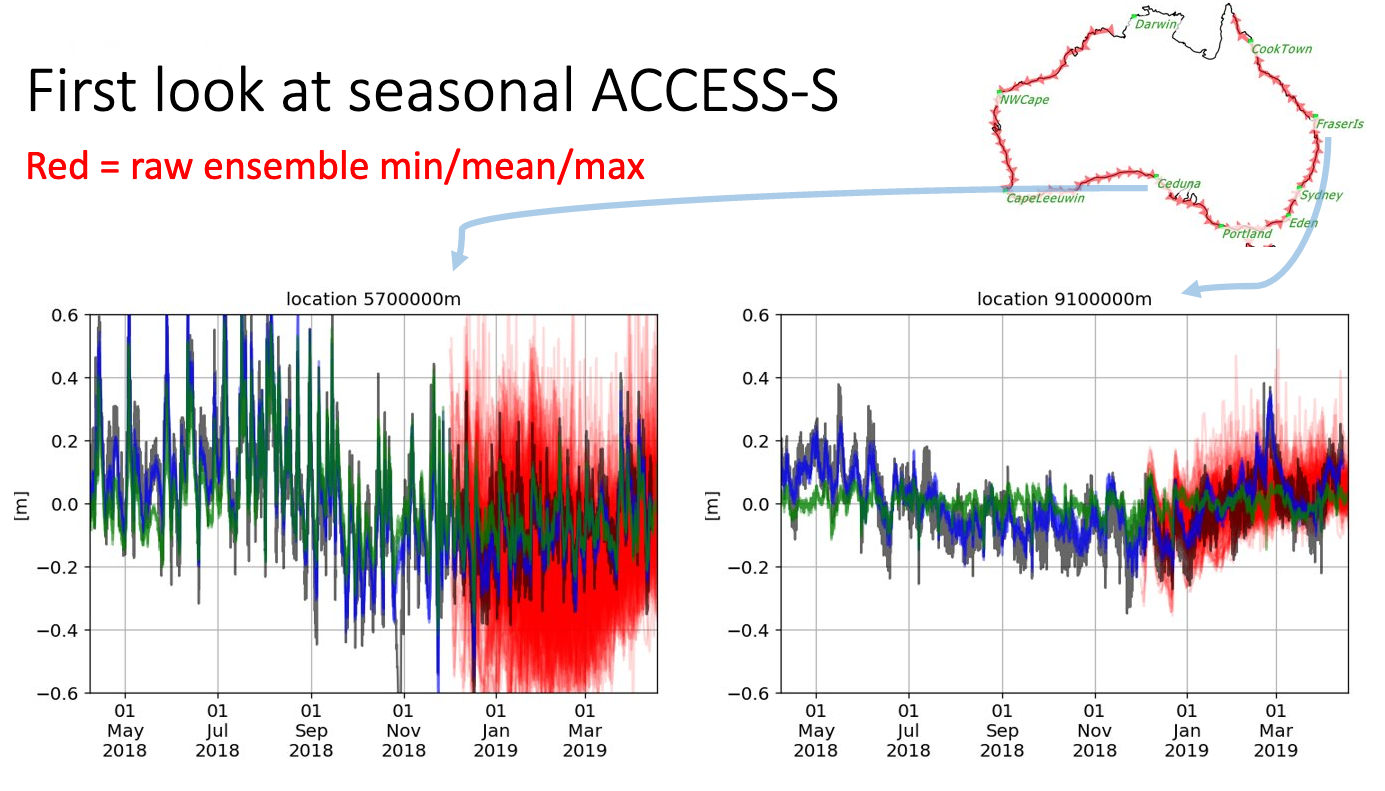
\includegraphics[width=120mm]{figures/images/spectra_cartoon_1.png}
\caption{Conventional decomposition concept: mixed sea level spectra comprising discrete tidal `lines' and red turbulent continuum.  Implementation of this concept has ramifications for sea level forecasting.}
\label{fig:SPECTRA_CARTOON}
\end{center}
\end{figure}


Viewing sea level as a stationary set of harmonics is at face value quite at odds with a view of the ocean as a turbulent fluid.   In that sense, Gallison's portrayal of physics as `neither unified nor splintered into isolated fragments' \citep[pp 782]{Galison:1987wh} is apt.  Thus also is Peterson's assertion of `\dots{} the fundamental plurality of \dots{} scientific practice' \cite{Petersen:2012tr}. 
\newpage
%--------------------------------------------------
\subsection{Operational Oceanography}
\label{S:operational_oceanography}

Mesoscale ocean prediction moved into operations across the early 2000s in a manner that lagged and imitated the path of NWP \citep{Harper:2008ub}. Operational oceanography is `big science' \citep{Petersen:2012tr} in the sense that it fundamentally relies on the coordination of large organisations, global networks and capital. \\
Starting in 1997, the international collaboration of the Global Ocean Data Assimilation Experiment \GODAE{} serves as a historical reference point:

\begin{quote}
The central idea of \GODAE{} - to demonstrate the feasibility and utility of real-time, global ocean forecasting - was based on the experiences of the meteorological community in \dots{} FGGE. \citep{Bell:2009uv}
\end{quote}


%-----------------%
\subsubsection{Ocean General Circulation Models}

Since \GODAE{}, Ocean General Circulation Models (\OGCM{}s) are a key component in operational oceanography.\\

An \OGCM{} simulates the physical ocean state via time-stepping a mixed boundary-/initial-condition problem.\citep{Griffies:2004vs}.\\
A distinction between \emph{resolved} and \emph{unresolved} scales is paramount.  `Sensitive dependence on initial conditions in this turbulent flow \dots{} severely limits predictive capabilities [and] motivates a formulation of averaged or mean field fluid equations' \citep[Sec 2.5]{Griffies:2004vs}.\\


Information cascades between turbulent scales places importance on sub-grid scale (SGS) parameterisations; and raises broad questions of representiveness.\\
Griffies perceives an \OGCM{} as representing the averaged motion of an infinite ensemble of hypothetical oceans; the imagined spread being proportional to the scales of SGS parameterisation.
Alternatively, Stevens casts \OGCM{}s into the class of geophysical `pseudofluid' simulations \citep{Stevens:2001kb}. Of which he notes comparisons with observational data are prone to interpretational nuance and are ``too often ad hoc, uncritical, and/or irrelevant''\citep[pp 286]{Stevens:2001kb}. \\

\begin{figure}[h]
\begin{center}
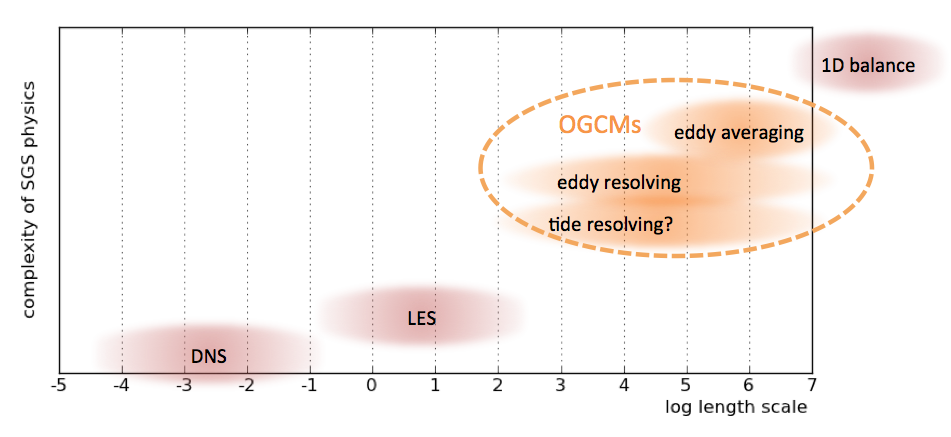
\includegraphics[width=120mm]{figures/images/model_types_schematic.png}
\caption{Schematic illustration of place of \OGCM{}s in terms of SGS parameterisation of the broad scale range of a turbulent ocean.  For reference, methods from turbulence studies are included: Direct Numerical Simulation and Large Eddy Simulation. Following \citep[fig 5.2]{Petersen:2012tr} and \citep{Stevens:2001kb}.  Inclusion of explicit tides is tentatively placed as a reduction of parameterisation without increased spatial scale resolution.}
\label{fig:models}
\end{center}
\end{figure}


Common to `big science' simulation practice \citep{Petersen:2012tr} an \OGCM{} embodies a large amount of collective and accumulated programming effort in many lines of computer code; too much for any one person to understand in detail. \\



%-----------------%
\subsubsection{Ocean Observations and Data Assimilation}
Data assimilation is the framework for combining information from ocean observations and the chaotic dynamics embodied by an \OGCM{}; usefully viewed from a Bayesian perspective\citep{Zaron:2011ft}.\\
Despite the growth of \GOOS{} \citep{Komen:1999ch}, the ocean is fundamentally under-observed for the purposes of physical state estimation.\\



Satellite-based ocean altimetry provides a data stream of special significance to contemporary ocean forecasting \citep{Fu:2001ub}. \\
Derivation of sea level quantities from satellite mounted radar instruments is particularly challenging in shallow water and near coastal boundaries \citep{Woodworth:2011bf}. 
Altimetry has directly enabled contrasting scientific developments in global tides (eg.\citet{Egbert:1996vr},  \citet{Lefevre:2011dg}) and mesoscale ocean variability (eg.  \citet{Wunsch:1998bq}, \citet{Chelton:vi}).

 
\newpage
\subsection{Ocean Tides}
\label{S:TIDE}

\BoxBegin
Tidal prediction is the oldest form of ocean prediction, and is still the most accurate \citep{Parker:2007wq}. \\
\BoxEnd

The language of ocean tides is particularly rich in ambiguous terminology and it is relevant to consider definitions closely.\\ 
Cartwright's \cite{Cartwright:2000tt} history is illustrative in never attempting to define what a `tide' is.  Implying that the \emph{history itself} is the only meaningful way to frame the scope of tidal science.\\
Pugh \cite{Pugh:1996uz} on the other hand addresses definition explicitly but casts a wide net; notably not locked to astronomy.  Any definition of tide ``\dots{} must emphasize this periodic and regular nature \dots directly related in amplitude and phase to some periodic geophysical force \dots''.\\

Contemporary geophysics places the Astronomical Tide Generating Forces \ATGP{} in a defining role.\\
Thus Henderscott \cite{Hendershott:1981ub} treats ocean tides as the subset of oceanographic long waves driven by the \ATGP{}. 
Although pointedly making a distinction between dynamics and `practical tide prediction', his treatment of the `ad hoc radiational potential'\cite{Munk:1966ts} is indicative of the fuzziness such a split.\\
Foreman \cite{foreman:2012perscomm} considers the core characteristic of tidal sea level is a response to the forcing of the tidal potential.   A similar emphasis is seen in Flinchim and Ray's \citep{Flinchem:2000kp} discussion.\\


This is the setting in which many instances of ostensibly oxymoronic terminology appear.
Discussion of \emph{non-stationary} tides \cite{Ray:2011tj}, \emph{quasi-periodic} tidal phenomena \citep{Flinchem:2000kp} or \emph{storm} tides \cite{Horsburgh:2008gw} oestensibly clashes with the perspective of conventional harmonic analysis.  The existence of such rich terminology highlights the need for semantic care in this area.\\



%-----------------%
\subsubsection{Common Foundation of the \ATGP{}}
Reference to the \ATGP{} is the common foundation to tidal methods.   

\begin{figure}[h]
\begin{center}
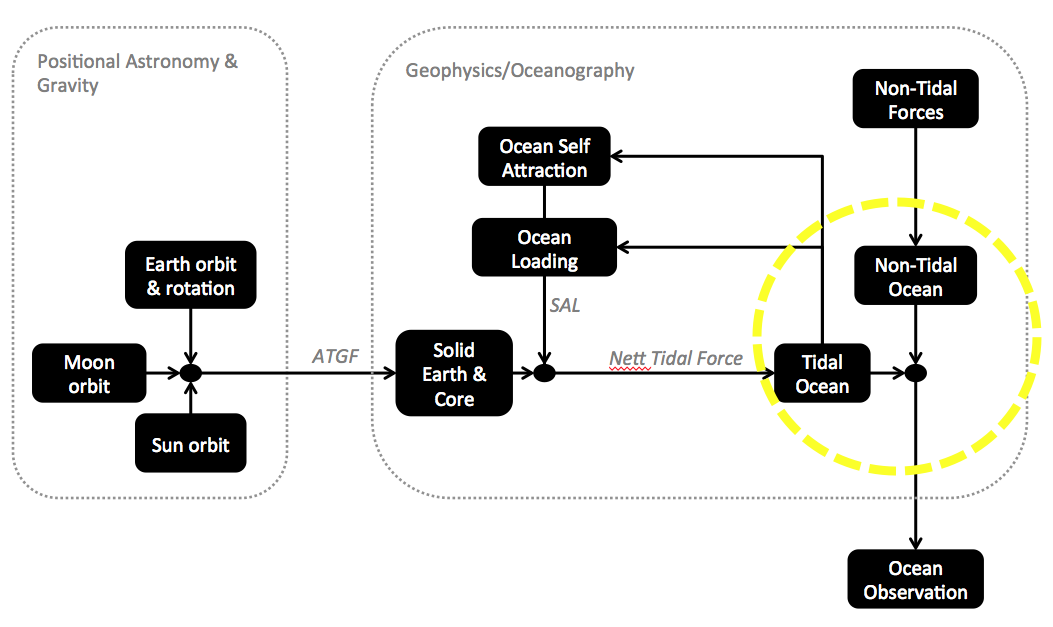
\includegraphics[width=120mm]{figures/images/tidal_force_flowchart.png}
\caption{Ocean tide flow chart (following Agnew \citep{Agnew:2011ub}.  Reference to the \ATGP{} is common to all tidal methods, whilst the distinction between Tidal/Nontidal elements can differ markedly.}
\label{fig:TIDE_FORCE_FLOW}
\end{center}
\end{figure}


If the gravity field is defined as a scalar potential in space $\Delta V=0$ \citep[sec 5.3.1]{Urban:2013vl}, a specific subset due to bodies external to the Earth, but excluding components acting uniformly over the Earth's surface, is termed the \ATGP{} or $V_T$.\\
Noting that various conventions exist \citep[sec 6.5]{Anonymous:2004tm}, $V_T$ relevant to ocean dynamics is formulated in geocentric coordinates following \cite{Cartwright:1973em} and \cite{Desai:2006wo}:

\begin{equation}
\label{E:VT}
\eta_{eq} = \frac{V_T(t,\theta,\lambda) }{g} = \sum_{n=2}^{\infty} \sum_{m=0}^{m=n} M_{nm} P_{nm}( \sin(\theta) ) \text{Re} \left [ c^{*}_{nm}(t) e^{im\lambda} \right ]
\end{equation}

Of itself, Equation \ref{E:VT} asserts nothing specific about causation, astronomy or ocean dynamics.\\
It is conventional to define $V_T$ normalised by standard Earth gravity $g$ as the \emph{equilibrium tide} $\eta_{eq}$ with units of height; for instance \cite[Eq 9.8.3]{gill1982atmosphere}. Use of this term unfortunately invites confusion with an actual ocean elevation - which it is not.\\


\begin{figure}[h]
\begin{center}
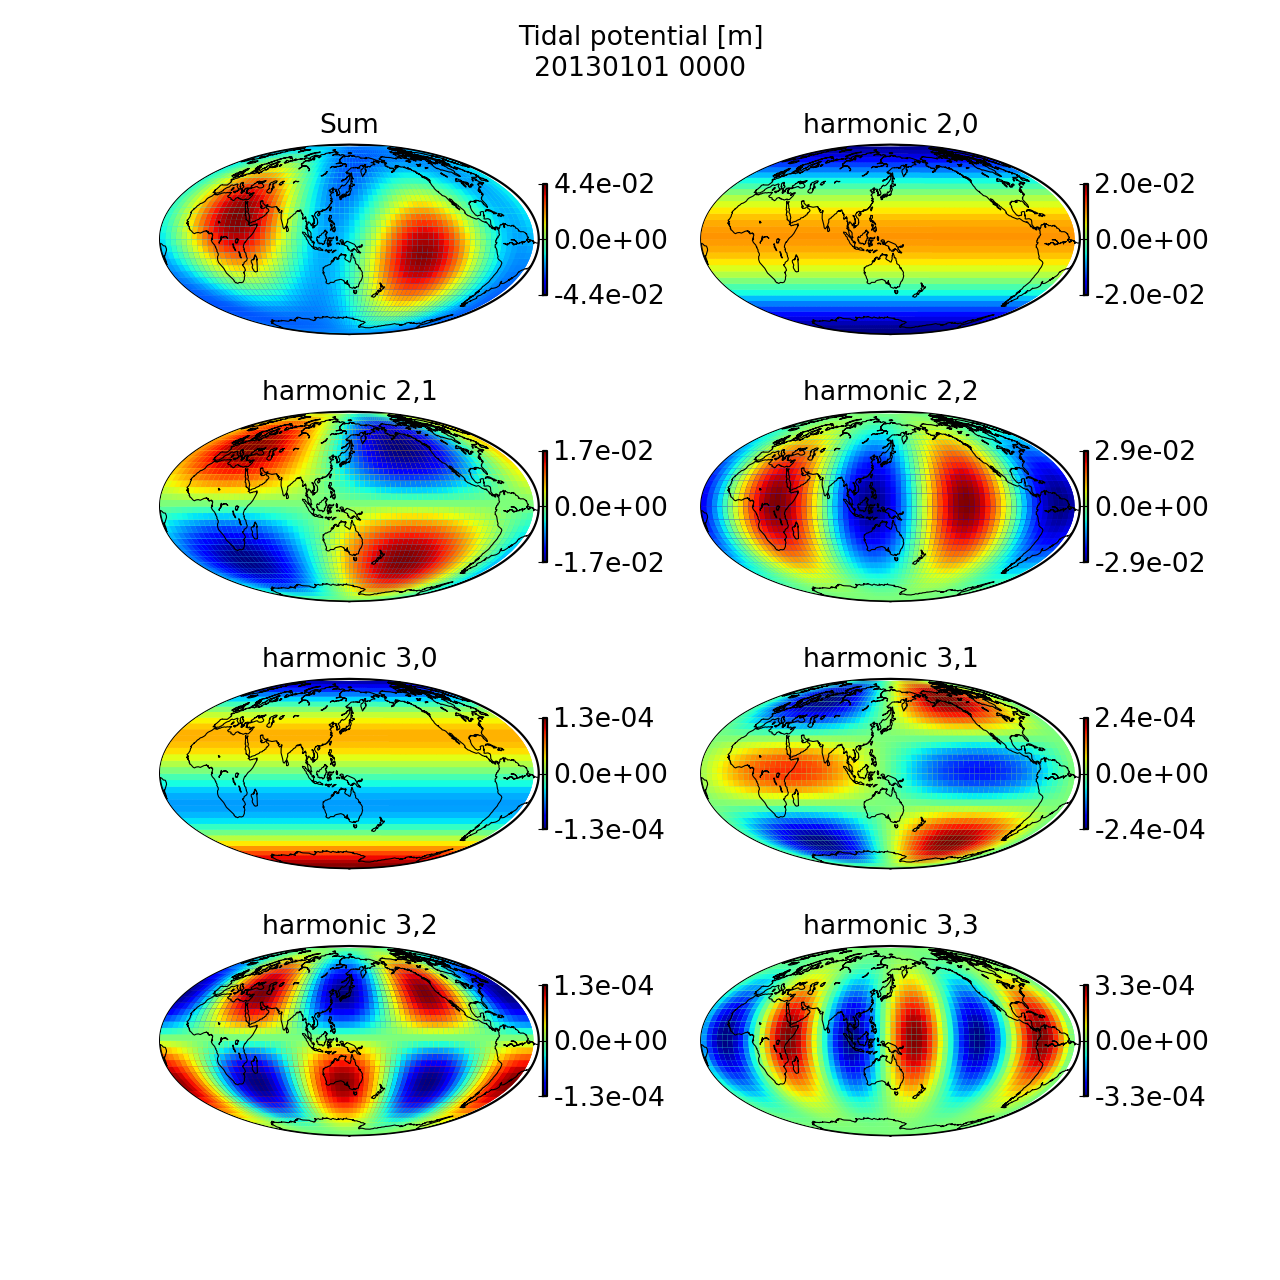
\includegraphics[width=120mm]{figures/images/tidal_potential_spatial_20130101_0000.png}
\caption{Snapshot of global $\eta_{eq}$ field illustrating spatial decomposition into spherical harmonics.  Note the wide variation of relative magnitude}
\label{fig:VT_EG}
\end{center}
\end{figure}


\begin{figure}[h]
\begin{center}
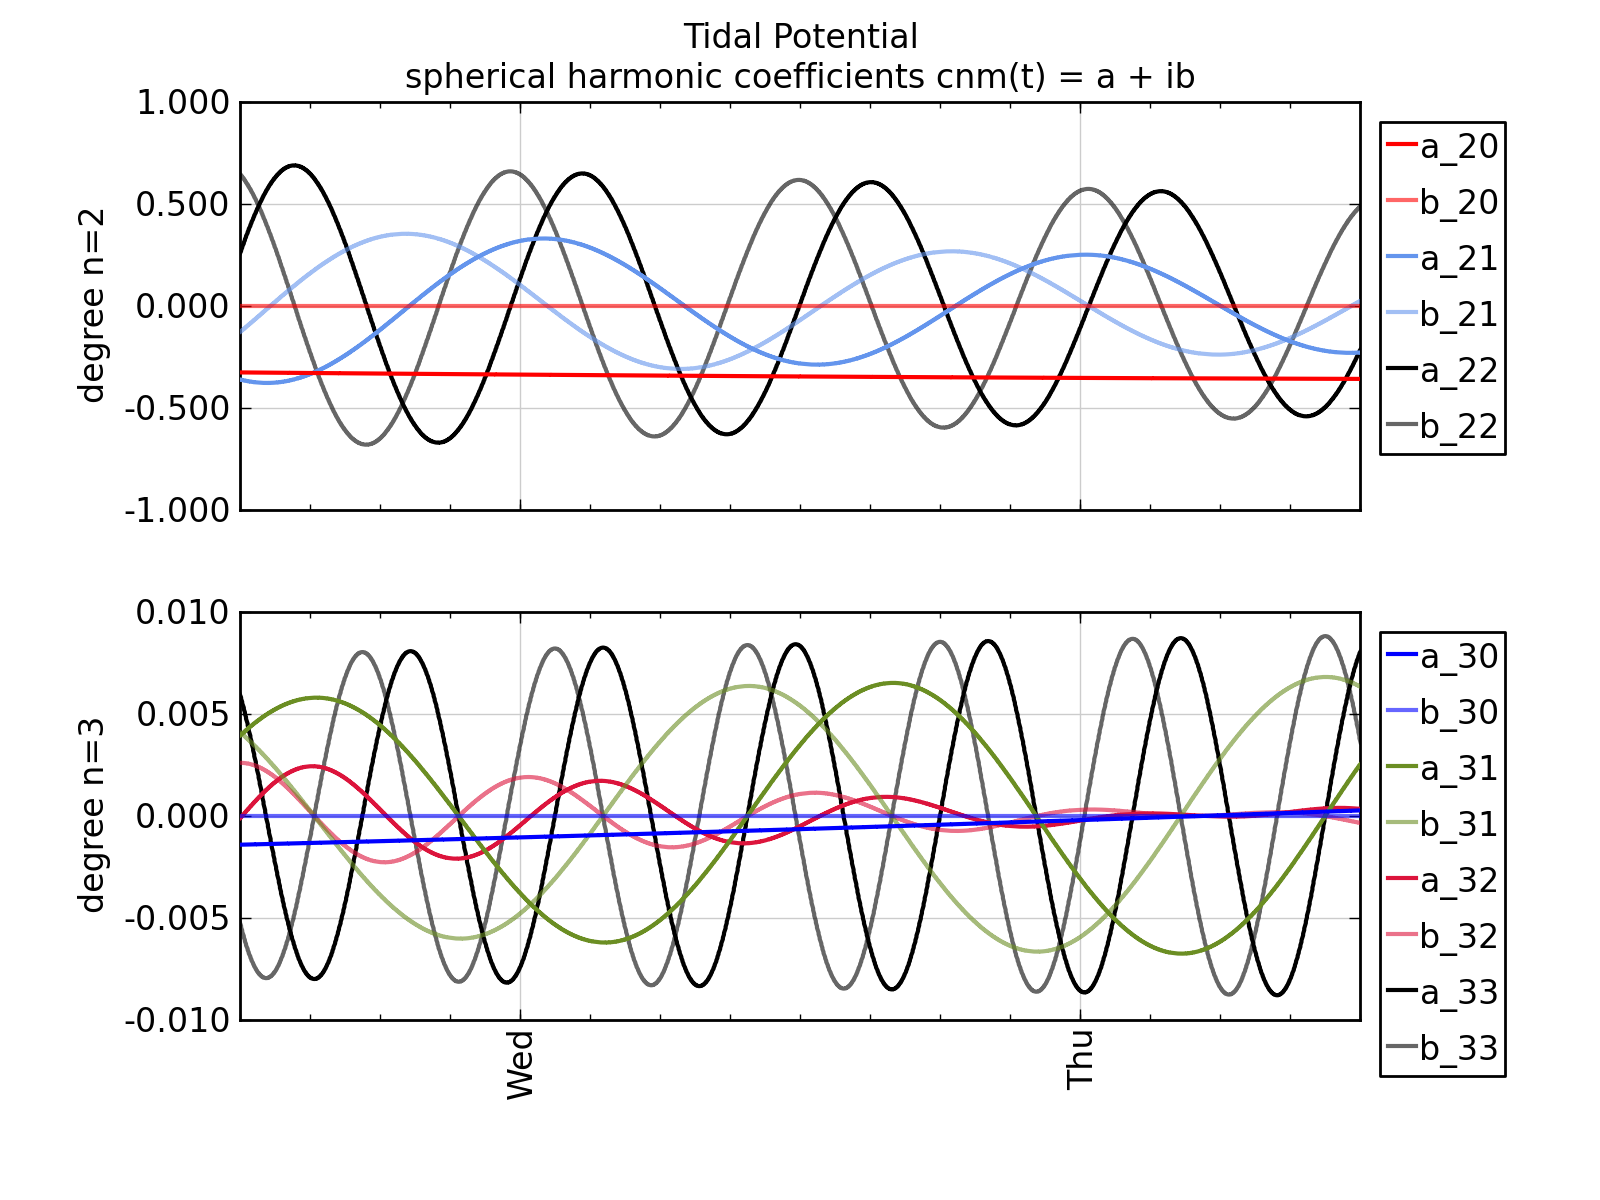
\includegraphics[width=120mm]{figures/images/tidal_coeff_timeseries_2days.png}
\caption{Snapshot of time varying coefficients $c_{nm}(t)$. Derived based on ephemerides output of DE421 utilising the software tools provided by NASA \cite[p]{Anonymous:vo}  In the upper panel, classification of $c_{2m}$ into long, diurnal and semi-diurnal `species' is evident.  Note the much smaller magnitude of higher degree harmonics.}
\end{center}
\end{figure}

Positional astronomical information is supplied from ephemerides \citep[Section 8.1]{Urban:2013vl} of which there are two broad classes: analytical and numerical \citep{Wenzel:1997kn}.\\
An analytical ephemeris is based on simple polynomial relations, valid for a given epoch.\\
Whilst analytical ephemerides are commonly behind ocean applications, numerical ephemerides are standard for non-oceanographic purposes and since the 1980s have been generated using data assimilative approaches\cite[sec 8.1]{Urban:2013vl}. The `current best estimates' for the orbits of the Moon and planets is DE421 \citep{Folkner:2008wm}. \\


%-----------------%
%\subsubsection{\ATGP{} Extras}
%\label{S:ATGP_extras}

The basic \ATGP{} development alone is not sufficient for ocean forecasting applications. In practice several nuanced but significant issues must be addressed.\\
In very brief outline:
\begin{compactitem}
\item Vertical movement of the ocean floor associated with the \ATGP{} is of comparable magnitude to the ocean tide and is quantitatively significant to ocean tide models \citep{Hendershott:1981ub} and \citep[pp.336]{gill1982atmosphere};
\item Elastic re-distibution of earth mass modifies the effective \ATGP{} felt by the ocean \citep{Agnew:2011ub};
\item Movement of ocean mass has an effect on the solid Earth, and reflexively on the gravitational potential acting on the ocean itself - lumped together as `self-attraction and loading' \SAL{}.  This can be a non-trivial issue for ocean models \citep{Ray:1998jl}, with qualitatively different approaches in common use \cite{Stepanov:2004up} \citep{Egbert:2002ug}.
\end{compactitem}



%-----------------%
%\subsubsection{Temporal Representation of the \ATGP{}}

Distinct \underline{temporal formulations} of Equation \ref{E:VT} are fundamental to tidal methods.  
In summary;
\begin{compactitem}
\item A tidal method based on $c_{nm}(t)$ derived from a numerical ephemeris could be said to be \emph{direct}.\\
\item Transformation of $c_{nm}(t)$ into frequency space is the basis for \underline{harmonic developments} of the \ATGP{}. Note the possible confusion of `harmonic decomposition' with `harmonic analysis'.
\end{compactitem}

% harmonic
A harmonic representation is given as per Equation \ref{E:harmonic} following \citep{Desai:2006wo} and \citep[Eq 13]{Cartwright:1971iz}.\\
\begin{equation}
\label{E:harmonic}
c_{nm}(t) = \sum_{k} H_{nmk} e^{-i( t\theta_{nmk})} = \sum_{k} H_{nmk} e^{-i( t\omega_{nmk} + \beta_{nmk})}
\end{equation} 
Equation \ref{E:harmonic} does not represent a Fourier series and the many hundreds of frequencies $\omega_{nmk}$ do not result in an orthogonal set of sinusoids.\\


Doodson \citep{Doodson:1921kt} introduced a novel and influential system of notation for specifying $\theta_{nmk}$ with a code of integers.  These provide a compact unique specification, and in practice \emph{definition} of frequencies relevant to tidal methods.


%-----------------%
\subsubsection{Ocean as an LTI System}
\label{S:LTI}
In stark contrast to \OGCM{}s, tidal sea level prediction practice is founded on treating the ocean as a linear time invariant (LTI) system \citep{Chatfield:2004uv} driven by the \ATGP{}.\\

Fundamental aspects of tidal methods were introduced by Laplace \cite[chpt 7]{Cartwright:2000tt}:
\begin{itemize}
\item spectral banded-ness of $V_T(t)$ (grouped as diurnal, semi-diurnal and long species) 
\item application of empirical time series analysis to characterise the outcome of complex global hydrodynamics. 
\end{itemize}

This is inherently a frequency-space perspective and relies on stationarity (time invariance). 
In fact, time stationarity is essential to the \emph{definition} of `tidal' in most operational settings.
Jay and Kukulka \citep{Jay:2003bj} suggest that tidal practice has ``$\dots$
solidified an opinion that tidal time series (particularly those of surface elevation) are basically stationary, with non-stationary components frequently being regarded as meaningless `noise'.''


\begin{align}
    c_{nm}(t)       \Rightarrow & \fbox{Global Ocean} \Rightarrow \mbox{observed response}                \nonumber 
\end{align}


All the complexities of ocean dynamics are hidden within the `black box' and are largely irrelevant, excepting that ``[by] an unfortunate coincidence \dots{} the frequencies of the free modes of ocean oscillation are intercalated with the frequencies of the tide-generating consitituents.\citep{Groves:1975ky}''



\begin{align}
\label{E:LTI}
H_{k}(\theta_k) \Rightarrow & \fbox{empirical LTI system} \Rightarrow \mbox{tidal ocean $f(\theta_k)$}  %\nonumber
\end{align}


Munk and Cartwright \citep{Munk:1966ts} named three foci for complications to practical implementation of direct relevance to the present research:
\begin{compactitem}
\item the background spectral continuum of ocean variation, 
\item non-gravitational phenomena that can be considered tidal and 
\item non-linear interactions.   
\end{compactitem}



%-----------------%
%\subsubsection{Tidal Harmonics and Alternatives}
%\label{S:formalisms}

There can be a wide gap between the practices of centres producing \underline{tide tables} and those used in other scientific settings.\\


Implementation of the LTI concept of ocean tide prediction falls in two categories: harmonic and response methods. \\
Recognising the common core, Le Provost \citep[chpt6]{Fu:2001ub} (unhelpfully) names both as instances of the `response' formalism. \\



Tide prediction is practically synonymous with \underline{harmonic methods} in operational centres.  These methods have a long history \citep{Cartwright:2000tt}\citep{Parker:2007wq} and are well embedded in the wider economy.\\
The practical value of harmonic methods reflect the power and \emph{predictability} of sea level variation occurring at tidal frequencies.  This value does not rely on explicitly describing ocean dynamics, and in fact the \emph{absence} of fluid dynamics is a key strength of harmonic methods.   


Essentially, harmonic methods identify an LTI system as per Equation \ref{E:cos}; illustrated by the simplistic assertion that 'the purpose of tidal analysis is to represent the water level \dots{} by a set of harmonics \dots{} having a specific amplitude and phase '\citep{PCTMSL:2009vy}.

\begin{equation}
\label{E:cos}
\eta_{tide}(t) = \sum_{k} f_k A_k \cos ( t.\omega_k + g_k + u_k)
\end{equation}

Significantly, the set of tidal frequencies is always truncated and often augmented with additional `compound' or `overtide' frequencies.\\


\begin{figure}[!h]
	\centering
	\subfloat[Harris-Fischer tide machine circ. 1921 \citep{Zetler:1987wf}]{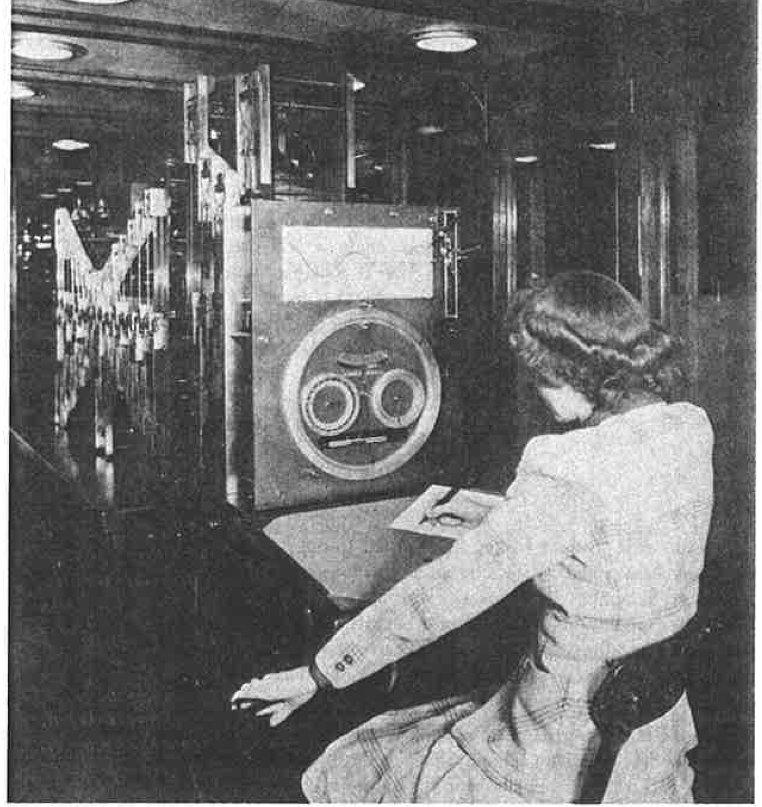
\includegraphics[width=50mm]{figures/zetler_tidal_computer_lady_1921.png}}
	\caption{Analogue tide machines embody harmonic prediction.  A finite set of fixed constants are dialled up for a port, and the handle turned to generate a prediction timeseries.}
	\label{fig:tide_machines}
\end{figure}


In linear algebra terms,  a harmonic analysis can be formulated as an overdetermined inverse problem:
\begin{equation}
\label{E:Axb}
\M{A} \V{x}=\V{b} 
\end{equation}
Where $\M{A}$ is a matrix of tidal timeseries basis functions, $\V{x}$ is the analysed tidal solution and $\V{b}$ is an observational record. Importantly, $\M{A}$ is neither orthogonal nor complete. Furthermore, overcoming the poor-conditioning of Equation \ref{E:Axb} has given rise to methodological conventions (eg cite{Foreman:2009bg}) often perceived as opaque and arcane.
Note that the `nodal corrections' or `satellite modulation' \citep{Foreman:2009bg} terms $f_k$ and $u_k$ in Equation \ref{E:cos} actually render the formulation more complex than a simple sum of sinusoids.\\
Harmonic analysis of sea level provides not only a powerful form of data compression \citep{Flinchem:2000kp} but importantly can give \emph{predictive} skill across lead times of many years.\\



%% non gravity
\label{S:nongravity}
The occurrence of non-gravitational influences of sea level at tidal frequencies can and does project from $\V{b}$ onto the solution for $\V{x}$.\\
For instance;
\begin{compactitem}
\item Non gravitational seasonal phenomena.  The meaning of harmonically analysed `\dots{} values of Sa and Ssa \dots{} [is] almost a philosophical question, based on one�s application' \citep[p122]{Parker:2007wq}.   Related terms include H1 and H2 in Foreman schedule \citep{Foreman:1977ua}\\
\item Higher frequency harmonics such as S1 and S2 can be primarily non-gravitational.  Including forcing signals from \NWP{} \citep{Ray:2003ui} used to drive ocean models.\\
\end{compactitem}

% response methods
Motivated partly by the contamination of non-gravitational effects, \underline{Response methods} \citep{Munk:1966ts} introduced in the 1960s form the primary alternative to the conventional techniques of harmonic analysis. The development was not driven by users of tide tables, but was rather a review to ``make explicit what the harmonic method does anyway''\citep[pp 540]{Munk:1966ts}.
Godin \citep{Godin:1991vx} describes this as `cross spectral analysis'.\\
It basically involves fitting LTI admittances using the empirical coherence of input and output timeseries. Inversion of an admittance function from tidal records can be classed as a discrete-time/continuous-frequency operation \citep{Percival:1998tw}.\\

The outcome of a response analysis is not a single admittance curve, but rather a small number of distinct curves; typically the semi-diurnal, diurnal and long-period tides associated with degree-2 spherical harmonics $(n,m) \in (2,2),(2,1),(2,0)$.\\

\begin{align}
\label{E:response}
g(\Delta t) + \dots &\Rightarrow & \fbox{empirical admittance curves $Z$} &\Rightarrow & \mbox{$\eta(\Delta t)$}  %\nonumber
\end{align}


% admittance
\begin{equation}
\label{E:Z}
\eta(t) = \sum_{n=2}^{3}\sum_{m=0}^{n}\sum_{k} H_{nmk} \text{Re} \left[ Z_{nm}(\omega)^*e^{-i(t\theta_{nmk})} \right] 
\end{equation}


% convolution
Determining $Z$ is not simply a matter of division in frequency-space.  Munk and Cartwright's \emph{convolution formalism} involves fitting \emph{smooth} complex-valued admittance $Z(i\omega)$ functions to each band-limited species via a convolution in time-space.\\
The \emph{bandwidth} of the tidal species is a relevant design consideration; for instance in Smith's \citep{Smith:1997ut} application to altimetry data.\\

% details
Certain fundamentals give rise to elaborations;
\begin{compactitem}
\item Nonlinear effects cannot be represented by a LTI model with only $\eta_{eq}$ as an input.  Given the importance of shallow water tides at the coast, somewhat inelegant multi-stage procedures evolved making use of `equivalent deep water ports' and paired and tripled product inputs \citep[pp 122]{Pugh:1996uz}.\\
\item Non-gravitational periodic sea level is excluded, but can be significant for tide tables.   This has lead to the early formulation of a somewhat ad-hoc `radiational potential' input (especially for S1 and S2). So-named due to an abstract connection with diurnal solar radiative fluxes.\\
\end{compactitem}

From a sea level forecasting perspective, the response approach modernised the formulation and increased the concreteness of the underlying physics, but in doing so hasn't ultimately provide anything more robust and simple for routine use in operational centres.
\begin{quotation}
$\dots$ the improvement in predictable variance is numerically small compared with the natural noise in sea level.   Because of this, and the fact that the Response Method is harder for a routine operator to grasp, it has never been adopted for ordinary tide-table production. It remains essentially a research tool for specialists. \citep[pp 198]{Cartwright:2000tt} 
\end{quotation}


%other
The convolution formalism is not the only viable implementation of the response concept and alternatives are described by Webb\cite{Webb:1974ke} and Desai \cite{Desai:1995je}.\\
% orthotide
More influential though is the \underline{orthotide} \citep {Groves:1975ky} approach to fitting Fourier series admittances.
In essence this is no different to Munk and Cartwrights convolution, but is an improved time-space formulation.  The resulting orthoweights have the attractive property of not being dependant on the number of components involved in any particular analysis, and subsequently share some of the characteristics of conventional tidal constants.
\begin{quotation}   
The use of orthotides may provide some benefits to the empirical determination of ocean tide models from a short duration of observations, but is otherwise unnecessary. \dots  polynomial and orthotide, and therefore convolution, approaches to modelling the smooth admittance function provided similar results as long as they are defined by an identical number of parameters.\citep{Desai:2006wo}
\end{quotation}


% nonstationary
Treatment of non-stationary tidal phenomena forms a scientifically important extension, eg \citep{Colosi:2006va} and \citep{Ray:2011tj}, but presently plays a very secondary role with regard to conventional sea level forecasts.\\
% wavelets etc
Tidal analysis techniques exist in the literature that are not immediately relevant to sea level forecasting; for instance, specifically tidal wavelet approaches to data analysis \citep{Flinchem:2000kp}.

%-----------------%
\subsubsection{Practical Use}
%\subsubsection{Admittance Curves and Constants}

% harmonics == admitance
Harmonic constants remain the lingua franca of ocean tide discussions.\\
Tidal constants are considered to represent samples from an admittance curve. For instance Smith\cite{Smith:1997ut} describes a transformation method.

% inference and smooth
An expectation that admittance curves $Z(\omega)$ should not contain discontinuities or sharp changes (the `credo of smoothness') is evoked to enhance the spectral content upon the \emph{synthesis} of tidal timeseries \citep[pp 268]{Fu:2001ub}).


Short tables of constants are indeed physically intuitive and facilitate simple error checking; a highly relevant consideration in the operational context.




%-----------------%
%\subsubsection{Forecasts and Filtering}

Contemporary operational centres employ tidal methods two distinct purposes: forecasting and \underline{filtering}. The distinction can and does lead to effectively inconsistent definitions `tidal' timeseries.\\
Tidal models by which altimetry observations are filtered (`corrected', `de-tided') \citep[table 3.2]{Scharroo:2011vd} have implications for ocean forecasts. Long-period tides \citep{Egbert:2003jd} and nongravitational tides \citep{Arbic:2005gv} are highlighted as points of special interest. 
In principle tide gauge observations could also be rendered consistent via appropriate de-tiding, for example \cite{Matsumoto:2000tg}.\\


\begin{figure}[h]
\begin{center}
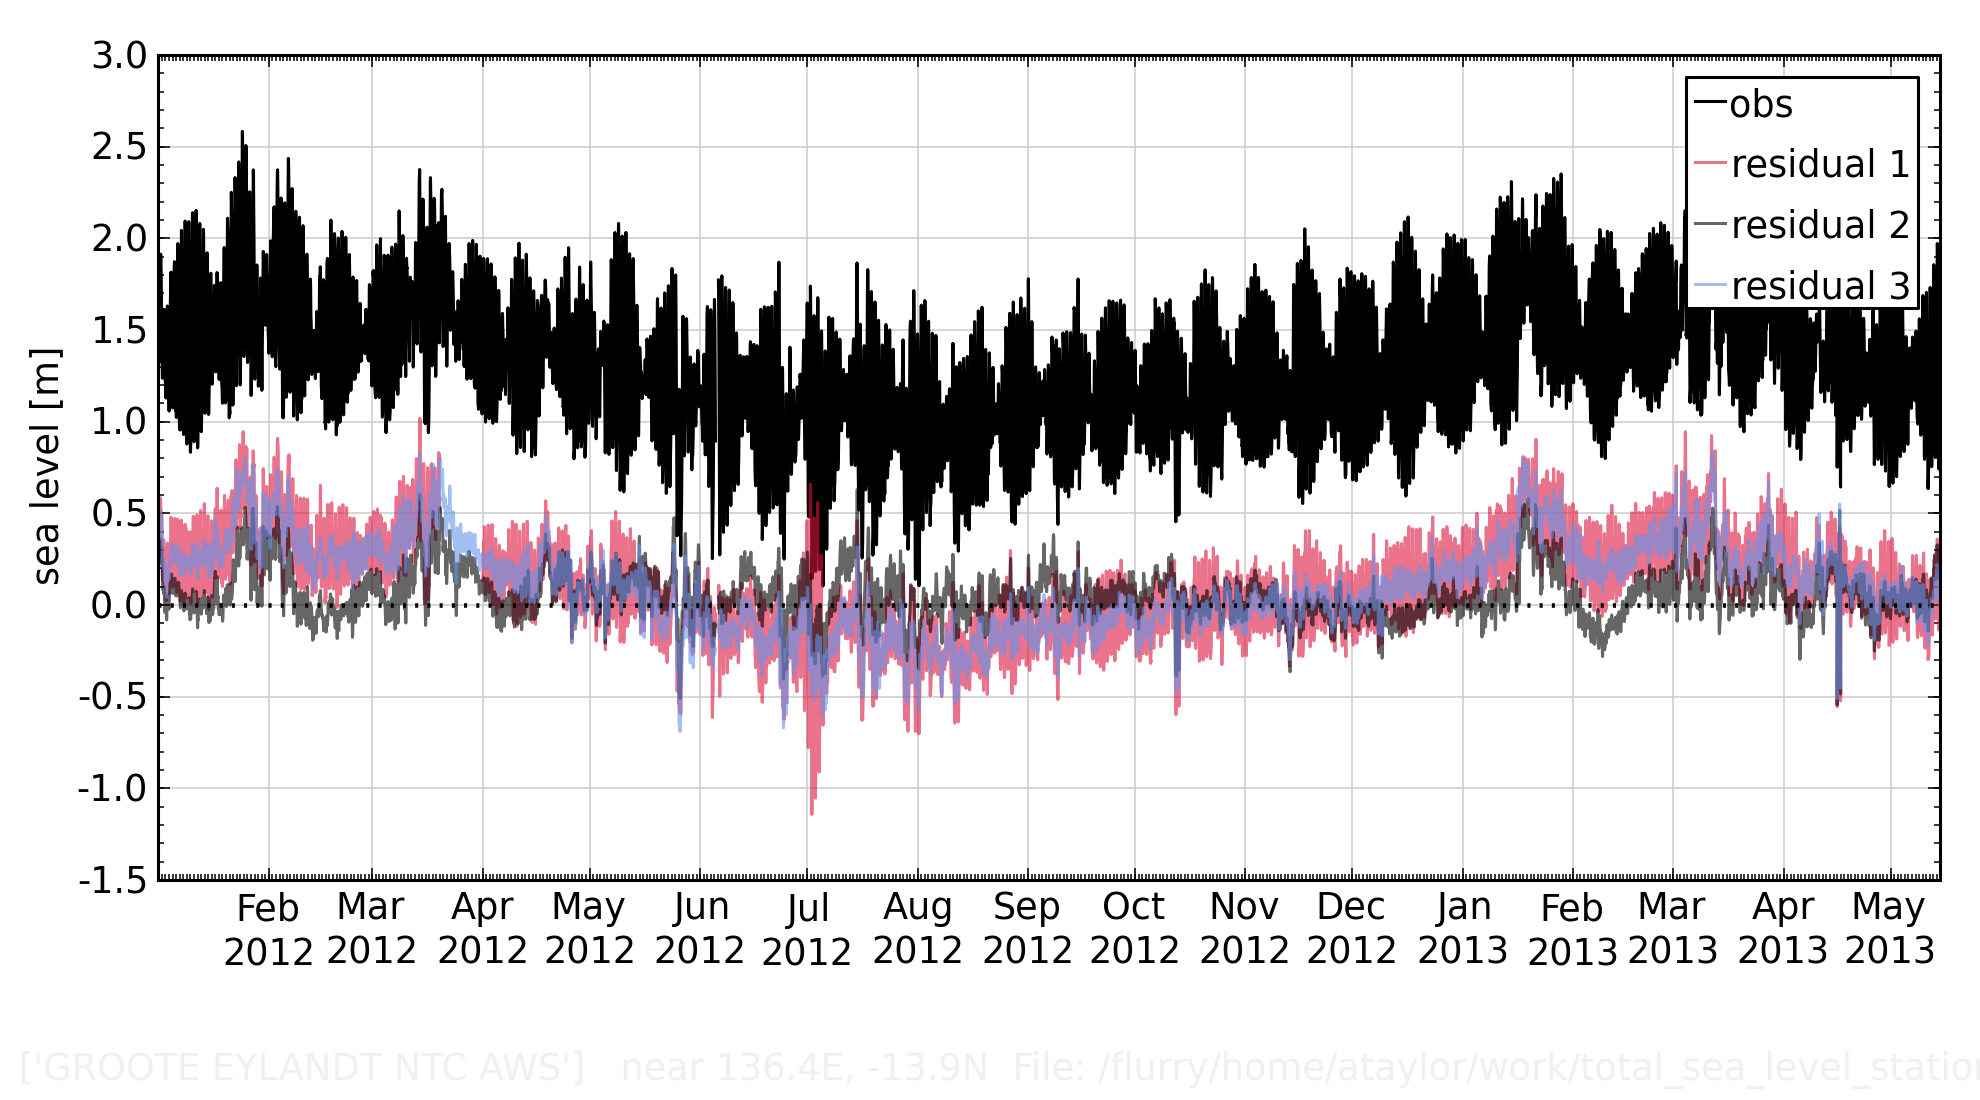
\includegraphics[width=130mm]{figures/images/diag_plot_014406_detide_compare_20120101.png}
\caption{Illustration of de-tiding observations by subtraction of tide predictions.  Different `residuals' result from alternative tide predictions: [1] regional gridded tide solution, [2] harmonic prediction and [3] harmonic prediction with specific non-gravitional harmonics removed. }
\end{center}
\end{figure}





In contrast to the situation with filtering, dynamical cause and effect are only relevant to stand-alone tidal forecast products insofar as they impact predictability. 
From a users perspective, tide tables simply forecast sea level and it is proper that the tide tables include all of the \emph{reliably} periodic signal regardless of cause.  \\
It is then not surprising that amongst Australian tide authorities treatment of long-period signals differs enough to warrant special review attention \citep{MHL:2013perscomm}.


%-----------------%
%\subsubsection{Global Tides and Atlases}
\subsubsection{Atlases and Data Assimilation}

In contrast to an \OGCM{}, the premise of a tidal atlas is to present maps of LTI admittance at discrete frequencies; conventionally as amplitude(co-range) and phase (co-tidal) diagrams for each `partial tide'. \\
This visualisation fits well with the concept of the tidal ocean as a linear sum of standing waves.   The long spatial scales and existence of spatial nodes places special importance upon \emph{amphidromes} - nomenclature introduced by Harris in the late 19th century \cite[pp 119]{Cartwright:2000tt}.  
Existence and placement of amphidromic points is an important visual metric employed to assess tidal model results \citep{foreman:2012perscomm}.  \\


% Meaningful tidal atlases existed prior to altimetry, most significantly that due to Schwiderski \citep{Schwiderski:1983ke}.\\


Coordinated development of improved tidal atlases with specific performance requirements formed a significant component of altimetry missions in the 1990s.
\begin{quotation}
\dots{} effort quickly split into two main approaches: the so-called empirical approach based on the direct analysis of the altimetry sea level time series \dots{}, and a modelling approach based on hydrodynamic and assimilation models. Later on, the interaction between the two approaches \dots{} was a key factor for the overall success in improving tidal prediction accuracy and reaching the [mission] requirements \cite[pp394]{Lefevre:2011dg}.
\end{quotation}

Global tide models play a role well beyond the purposes of sea level forecasting per se.  For instance in the quantification of gravity effects, orbit determination, earth rotation and even the definition of coordinate systems \citep{Anonymous:2004tm}.\\


Modern tidal atlases are in close agreement with regard to global patterns, but characteristically differ at the shallow water margins; the very location of direct interest to sea level forecasts.  Figure \ref{fig:tpx_cross} illustrates the fact that modern global tide models typically agree within about 0.02m in the deep ocean, but can differ substantially in coastal and shelf regions. 


\begin{figure}[h]
\begin{center}
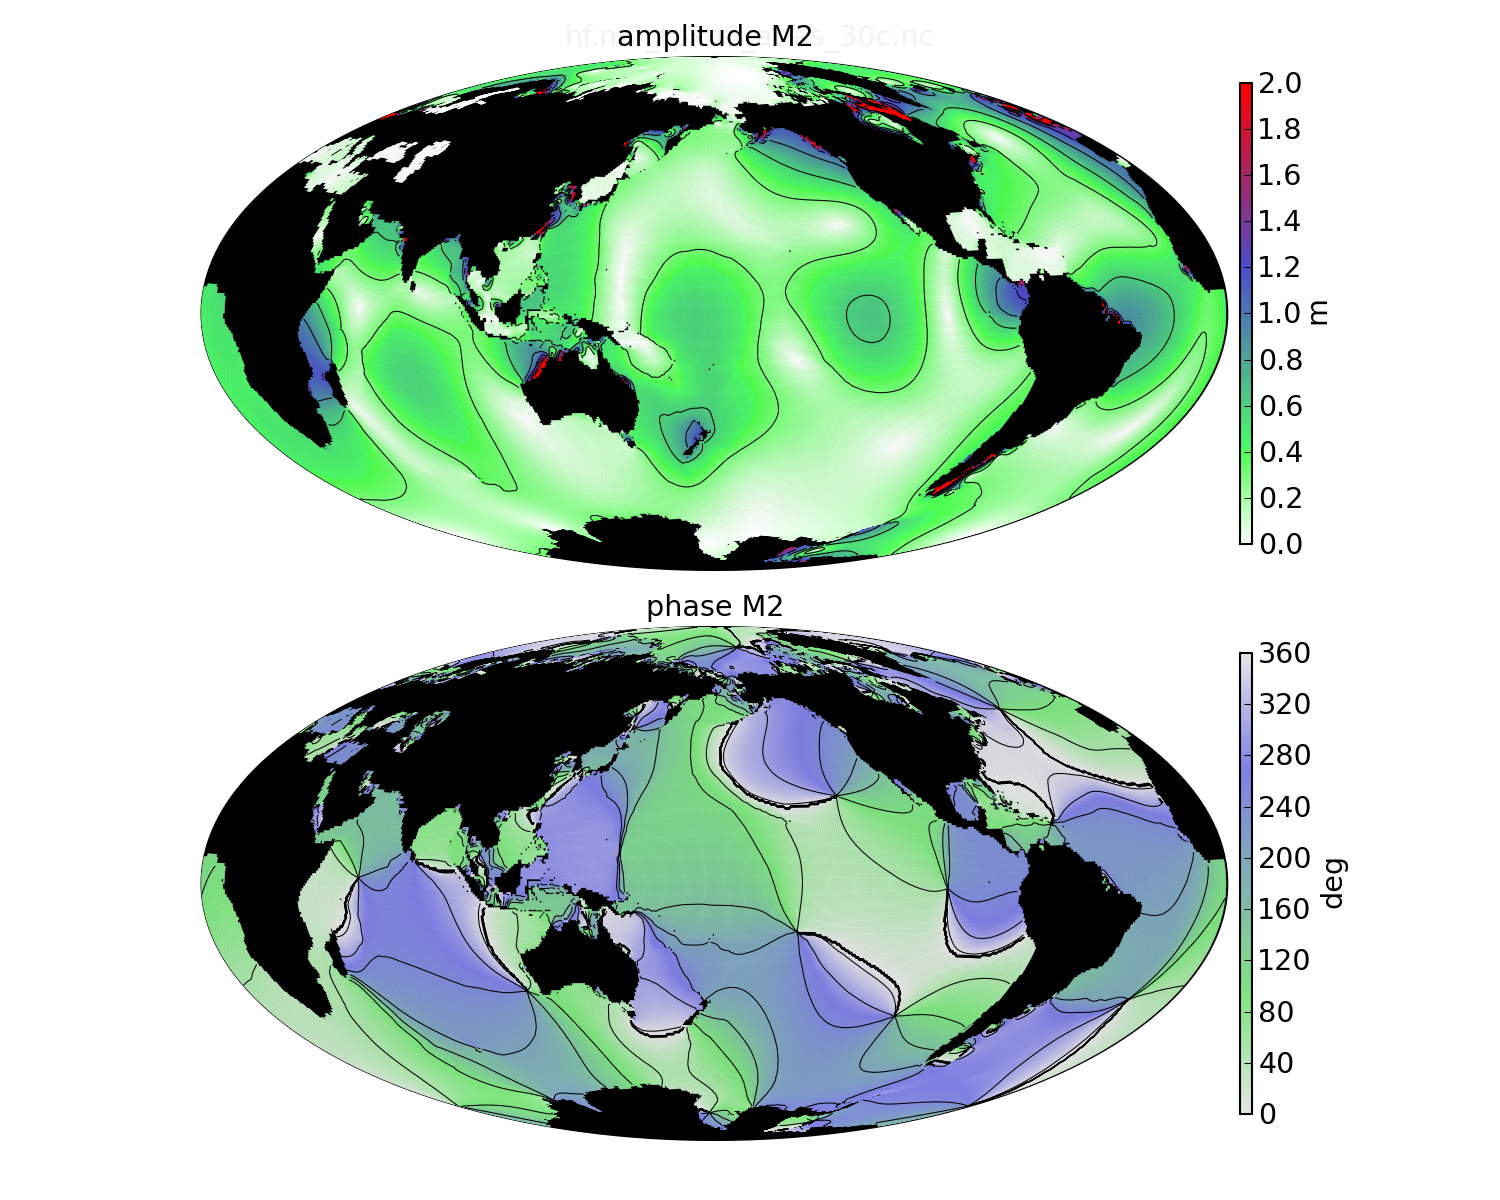
\includegraphics[width=130mm]{figures/images/global_m2_tpx08.png}
\caption{Example tidal altas showing cophase and corange diagrams for a single tidal component M2.  Data source TPX08 \cite{Egbert:2002ug}  }
\label{fig:atlas}
\end{center}
\end{figure}


\begin{figure}[h]
\begin{center}
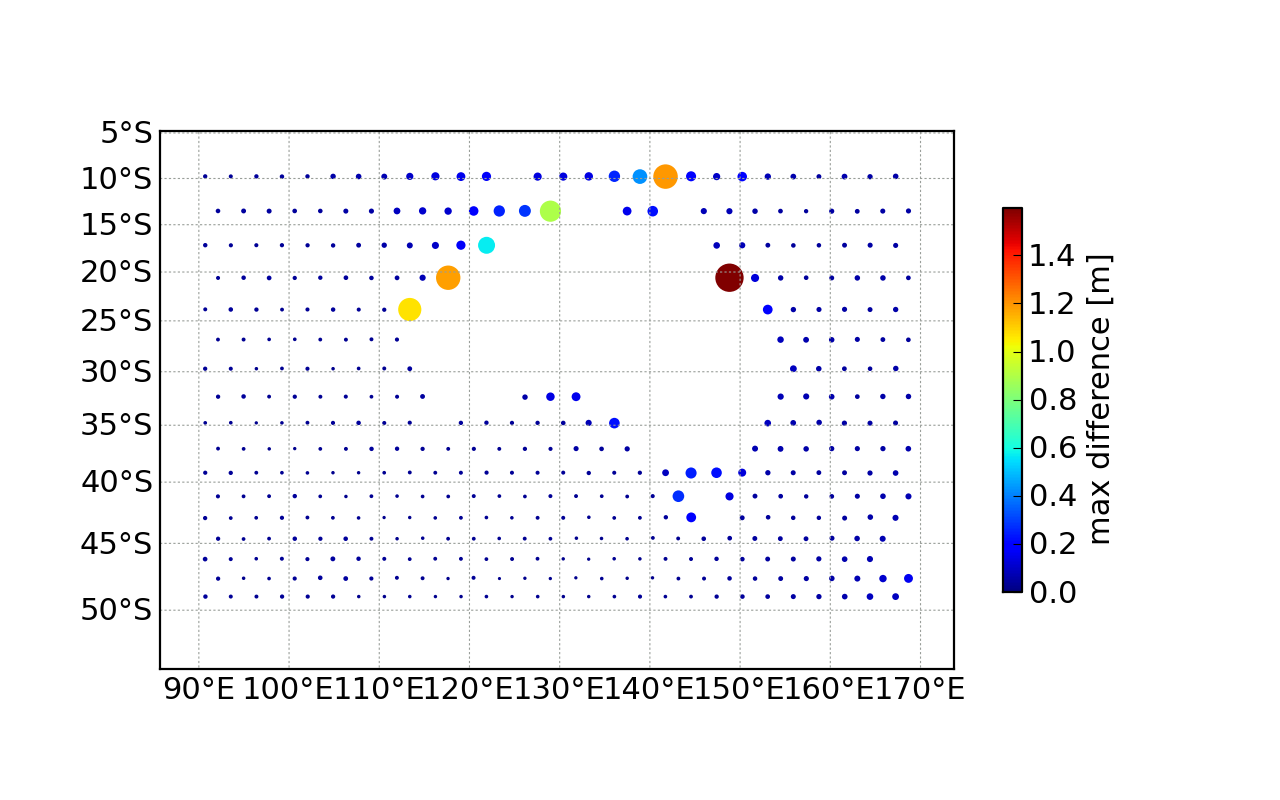
\includegraphics[width=110mm]{figures/images/map_tide_differences_tpx_xovers.png}
\caption{Maximum difference between tidal timeseries for 2012 at topex cross-overs near Australia.  The different solutions agree very closely in deep water, whilst the significance of shallow water effects are apparent.  Models included: CSR04\citep{Eanes:1996tr}, FES04\citep{Lyard:2006ir}, DTU10\citep{IMPROVEMENTOFGLOBA:2010tu}, GOT47, GOT48\citep{Schrama:1994vr}\citep{Ray:1999vm} }
\label{fig:tpx_cross}
\end{center}
\end{figure}


Understandably, global tidal atlases have focussed attention on linear deep water signals and have poorly represented or ignored coastal nonlinearties.  The nonlinear M4 signal is perhaps the only such partial tide to be included in global atlases and is observable with altimetry \cite{Ray:2010jm}.\\



As a forecast product, tidal atlases have nothing like the broad economic integration of conventional coastal tide tables.  The Australian Bureau of Meteorology does not promulgate official tide predictions away from insitu observation locations. \\




%-----------------%
%\subsubsection{Tidal Hydrodynamics and Data Assimilation}

In contrast to gauge-location predictions, global tidal atlas can not be purely empirical due to observation sparsity.\\
Instead observations are combined with hydrodynamics, the Laplace Tidal Equations (LTE) \citep[9.8]{gill1982atmosphere}citep{Hendershott:1981ub}, to produce data assimilative solutions.   
Compared to the dynamics represented within an \OGCM{}, these tidal hydrodynamics simulate a more `aggregated' psuedofluid in that the processes contained within parameterisations are have a higher degree of complexity.\\

Linearised LTE can be solved in spectral form.  The resulting computational efficiencies are important in facilitating data-assimilation methods \cite[pp184]{Egbert:2002ug} and \cite[pp395]{Lyard:2006ir}.\\


Whilst numerically solving the LTE is comparatively cheap, significant uncertainties prevent a direct `free' forward model from producing accurate forecasts. 
Solutions are complicated by the sparsity of observations ``$\dots$ open boundary conditions and bottom topography, the need for approximate parameterisations of dissipation in the tidal equations, solid earth effects, and the effects of ocean stratification \dots{}'' \citep[183]{Egbert:2002ug}. These same complications mean that ``global tide models are an ideal testing ground for the hydrodynamical cores of numerical \OGCM{}s, and for ideas about drag and dissipation ''\citep{Arbic:2004wz}.




Schwiderski's pre-altimetry solutions applied `hydrodynamic interpolation' to harmonic constants from mainly coastal tide gauges;  in hindsight an application of data assimilation \cite[pp822]{Egbert:1994wz}.\\
A comparative description of data assimilation methods in the context of tide models is laid out by Egbert and Bennet \cite{Egbert:1996vr}.\\   
Summaries that categorise the many global tide models on the basis of design choices, parameterisations and data assimilation methods are given in \cite{Ardalan:2008gs} and \cite{Matsumoto:2000tg}. \\



The tidal view of the ocean as a LTI system driven by the \ATGP{} is very useful, but with the caveat that ``the ocean is a physically complex and noisy filter.  In consequence, tidal harmonics are not strictly constant \citep[197]{Ray:2010jm}''.\\

Depth integrated LTE models effectively parameterise the effect of internal mechanisms on surface elevation.  This notably includes conversion from the barotropic to higher baroclinic modes \cite[pp121] {gill1982atmosphere}. \\
\begin{quotation}
Barotropic tides generate internal tides, and internal tides in turn feed back onto the barotropic tides. Inferences from altimetry-constrained barotropic tide models show that about one-third of global tidal energy dissipation occurs in regions of rough topography, where internal tides are generated \dots{}. Internal tide generation thus acts as a damping mechanism for the barotropic tides.\citep[pp22]{Arbic:hy}
\end{quotation}

For sea level forecasting, internal modes are ostensibly of interest insofar as they impact the prediction of surface elevation.  Internal waves at tidal frequencies do have an observable direct surface signature albeit relatively small \cite{Ray:2011tj}.\\


The very coarse parameterisations of baroclinicity in tidal models is in stark contrast to the primary focus of \OGCM{}s.   



% segue into OGCM
%--------------------------------------------------
%--------------------------------------------------
\subsection{Tides and \OGCM{}s}
\label{S:tides_ogcm}
To date \OGCM{}s in the \GODAE{} heritage have focussed on nominally \emph{nontidal} ocean dynamics, with de-tided sea level observations playing a unique role.\\


From that background, recent publications indicate a motivation towards more dynamic representation of the effects of ocean tides.   This is indicative of pervasive goal across numerical simulation practice to increase model concreteness by reducing the role of parameterisations \cite[section 5.3]{Petersen:2012tr}; a reduction of system aggregation \citep{Stevens:2001kb}.\\
Similarly, Griffies describes the ``general trend in ocean climate modelling towards reducing many of the common approximations'' \citep[pp20] {Griffies:2004vs}.
It could be said that the modelling community perceives parameterisations as a compromise that should ideally be replaced with explicit physics when computing power allows.  In spite of this, operational justification is a separate matter.


%-----------------%
\subsubsection{Nominally Nontidal \OGCM{}s}
\label{S:nontidal}

\BL{} is a nontidal system in that no gravitational body forcing associated with the \ATGP{} is applied.   Subsequently, assimilated observations of sea level are corrected (filtered) using pre-computed global tide models.  The state variable quantifying surface elevation carried by the model is termed sea level anomaly (SLA) which in itself is a rather abstract quantity. Using Stevens' nomenclature, \BL{} simulates an aggregated pseudofluid system with a qualified relationship to the actual ocean.


% split 
Timescales for depth-integrated barotropic and depth-dependant baroclinic ocean state are quite distinct and the design of \OGCM{}s have been influenced by this distinction. \\
%rigid ild
One approach has been to make the so-called `rigid-lid' approximation \cite[pp128]{gill1982atmosphere}. 
The rigid-lid by definition cannot represent explicit barotropic tides, and has other ramifications for ocean forecasting \cite[pp19]{Griffies:2004vs}.\\


% split explicit
A compromise strategy employed in \MOM{} (and other \OGCM{}s) is the so-called `split-explicit' scheme.    
In essence, cheap shallow-water barotropic dynamics are timestepped many times for each relatively expensive update of the full depth-dependant ocean state.  \\
Thus \MOM{} at face value is capable of representing barotropic surface tides.   However, there are several high level arguments against doing so.\\
One reason is the aims to which the model is being employed.  Much of the development of \OGCM{}s has been focused at climate times-scales, tipping the balance of away from the accuracy of high frequency sea level signals.   
Furthermore, in comparison to highly tuned tidal altases, simple and general barotropic can't be expected to achieve similar skill.\\

Filtered altimetry observations provide great value in observing and forecasting mesoscale eddies.
Treating tides as noise is reasonable insofar as the effects on the mesoscale structure are small relative to other source of error.\\

Decomposition of the dynamics into tractable categories for simulation is not aggregation per se, but it certainly does have implications for the role of parameterisations.  \\

From the perspective of \emph{users} of ocean forecasts there is basically no inherent value in decomposition.   
 
%-----------------%
\subsubsection{Motivation to Explicitly Resolve Tides}

As processing capacity increases, compromises imposed by past computing limitations are re-contextualised.   Inclusion of explicit tides within \OGCM{}s is increasingly affordable from a computational perspective.

With developments to date, exploration of this possibility has been directed primarily at the influence of barotropic tides on the baroclinic structure of the ocean state.   \\


% tides <-> baroclinic
Barotropic tides do interact with the baroclinic structure of the ocean, which conversely impacts the behaviour of barotropic waves and the \emph{non-constant} \citep{Ray:2010jm} nature of tidal constants.\\

Beyond the general simulation goals of model concreteness, it is the possible significance of barotropic/baroclinic interactions for global circulation that provides the primary motivation for considering explicit resolution of tides within \OGCM{}s.   



%-----------------%
\subsubsection{Temporal Formulation of Tidal Forcing}
\label{S:numerical_impl}

The astronomical tidal forcing can be conceptualised as a relatively smooth global surface field that varies in time. 
Perhaps the most significant numerical implementation consideration is how this time variation is formulated.\\


At face value, the \underline{direct formulation} provides the most unmediated and accurate representation of $\eta_{eq}$. Given spherical harmonics $(n,m) \in (2,0) , (2,1) , (2,2)$, the full global tidal forcing can be pre-computed $c_{nm}(t)$ as 6 real valued time series and simple trigonometric functions of location.\\
This approach has the advantage of accurately representing the \ATGP{} and facilitates incorporation of best-practice pre-computed SAL corrections \citep{Egbert:2002ug}. \\
Furthermore, this approach could offer consistent numerical formulation with other barotropic forcing fields.\\


On the other hand, some programatic inconveniences and risks are introduced. 
The input time series must be extracted from the ephemerides at timings to suit each particular simulation.  Furthermore, the extraction process is relatively opaque and would require cross-checks to mitigate the risk of non-fatal errors arising for file dependancies (e.g. incorrect dates).\\
Direct forcing is apparently not as common in the ocean literature as in gravity related studies.   
One instance of forcing a global hydrodynamic model directly is described by Weis and Sunderman \citep{Weis:2008ex} - notably in an non-operational setting.\\\



In contrast, a \underline{harmonic formulation} of $c_{nm}(t)$ for the same range of spatial harmonics requires the specification of many constants for each \emph{temporal} harmonic to be included.  
Hundreds of harmonic components \citep[pp3]{Desai:2006wo} would be required to match the spectral content of an equivilant direct formulation.\\

In practice only a small number (often 8) of the most powerful spectral clusters are specified as `primary constituents'.  
Truncation is based on the relative power of tidal lines within the harmonic development and subsequently requires nodal adjustments (as per Equation \ref{E:Axb}).

Programatically the harmonic approach facilities some attractive simplifications.  
After the specification of a small number of constants, the temporal variation can be cheaply calculated within the ocean model via only a few lines of code.   
For relatively short simulations ($\ll$ 1 year), the nodal corrections are reasonably treated as fixed.   This situation is amenable to de-bugging and has no external dependancies.\\
It is also a relevant consideration that assessment of tidal output is conventionally based on harmonic fits to these same primary constituents.\\

Arbic et al \citep{Arbic:2010us}, apply body forcing using the temporal harmonic representation.  In what appears to be common approach the authors describe developing their implementation via a progressive addition of temporal harmonics: no tides, M2-only, 8 primary constituents.  Treating M2 separately facilitates interpretation and comparison to other literature; including theoretical developments of single frequencies and tidal atlases.



%MOM
The public distribution of \MOM{} includes a very simple module for representing tidal body forcing in a manner suitable for climate simulations\cite[pp263] {Griffies:2008vh}.\\
The eight most powerful constituents (frequency clusters) from $\eta_{eq}$, due to only spherical harmonics $(n,m) = (2,1) , (2,2)$, are written with fixed harmonic amplitude.  SAL is simply parameterised with the scalar approximation. \\
Astronomical phase information is neglected altogether.
Schiller and Feidler \citep{Schiller:2007gk} worked around this gap with addition of a hard-coded astronomical argument offset valid for a particular epoch.\\
Tidal body forcing is written as a depth-independent horizontal term in the momentum equation evolved at the barotropic timestep.
This cheap barotropic code reflects the climate-simulation background of \MOM{}.  
By default, arbitrary forcing terms such as surface fluxes are held constant over iterations of the inner barotropic loop.  
Whilst this is a reasonable optimisation given relatively slow forcing timescales, it is not valid for $\eta_{eq}$ which varies powerfully and quickly.
By employing the temporal harmonic approach to representing the tidal force, $\eta_{eq}$ can be updated algebraically at the barotropic timestep, without requiring relatively expensive file input/output.\\




\subsubsection{Other Aspects of Formulation}
Beyond the basic \ATGP{}, there may be some prospect for translating forcing corrections from \emph{tidal} data assimilation models to an \OGCM{}. \\
The \underline{Generalised Inverse} (GI) \cite[pp345] {Zaron:2011ft} approach employed by \OTIS{} \cite{Egbert:2002ug}, draws an objective trade-off between observational and dynamic uncertainties; the ``inevitably approximate nature of the discretised dynamical constraints''\cite[pp155]{Egbert:1996vr}.  The inversion process involves determining adjusted forcing to achieve the optimal trade off.\\
Thus it is speculated that complementary use of \OTIS{} may be exploited to improve the representation of a stationary tidal signal in the time-stepping \OGCM{}.  \\


%OBC
Application of tidal forcing to a \emph{regional} prediction system raises the topic of open boundary conditions (\obc{}).  \obc{}s are of fundamental importance for limited area ocean models but review is considered beyond the scope of this document at present.\\


%-----------------%
\subsubsection{Vertical Mixing}

% climate mixing
An emphasis on improving the representation of \emph{baroclinic} circulation is apparent in \OGCM{} simulations implementing explicit tides.\\
Simmons et al \citep{Simmons:2004fi} are motivated to increase the concreteness of parameterisations with regard to the conversion of barotropic tidal energy.  Surface elevations were not the target of these simulations. \\


% schiller MOM
At timescales closer to those of operational forecasts, Schiller et al have also employed explicit tides within free-surface configurations of \MOM{}.  
Better representation of baroclinic mixing is again a primary motivation. 
Specifically, improved understanding of water mass structures \cite{Schiller:2004fv} and upper ocean circulation \cite{Schiller:2007gk} were cited as justifications for the implemention.  
Whilst the resolution of these configurations did not aim to resolve internal tide processes, explicit barotropic tidal currents enabled vertical mixing parameterisations to reflect spatially and temporally varying tidal effects.\\
In addition to the focus on mixing, surface level skill was evaluated against a coastal tide gauge and shown to offer some promise as a prognostic output \citep[Fig 2]{Schiller:2007gk} - apparently despite expectations.   
The issue of top-layer thickness limitations on surface elevation magnitudes highlighted by the authors does not directly apply to the contemporary \BL{} configuration of \MOM{}, which employs the $z^*$ coordinate \citep{Brassington:2012wm}.\\


%-----------------%
\subsubsection{Conversion Parameterisation}

% wave drag
Bringing astronomical forcing effects from `parameterised' to 'resolved' is a significant change with ramifications for parameterisation settings generally. \OGCM{}s parameterisation typically do not scale well.\\



Arbic et al \cite{Arbic:2004wz} discuss the `inordinately large' bottom drag values required by hydrodynamic tidal models and argue for the value of additional topography-based parameterisations.   
For example, the wave drag scheme described by Jayne \cite{Jayne:2001tr} is designed to spatially align barotropic dissipation over features such as mid-ocean ridges that are known to be source of internal tide generation.  Whilst a spatial concentration over internal tide generation locations is attractive - the relationship to vertical mixing may be misaligned to the extent that the energy cascade is non-local.  Internal wave propagation has a frequency/latitude dependance, with a qualitative transition from propagating to trapped occurring poleward of critical latitudes.  Furthermore `` the extent to which internal tides produce turbulence as they propagate away from their generation sites is not clear'' \citep[pp812]{Jayne:2001tr}.\\



It is notable that a related scheme is employed by the operational \emph{non-tidal} barotropic model employed for altimetry corrections (T-UGO, previously MOG2D)\citep{Carrere:2003cj}.  Model parameters, including a `internal wave' term, were tuned by means of a tidal simulation and comparison to tidal harmonics. \\


% schiller drag
The need to apply a special dissipation term to barotropic tides is also described by Schiller \citep[Eq 6]{Schiller:2007gk}.   This additional drag term was applied only within the barotropic loop and was designed via a tuning procedure but not described in detail.



% Arbic HYCOM
Arguably the leading tidal \OGCM{} developments described in the literature are those of Arbic et al. who have implemented a tidal version of HYCOM \cite{Arbic:2005gv,Arbic:2009hf,Arbic:2010us,Arbic:hy}.\\
Generally, the development procedure described involves a preliminary tuning of a spatially varying wave drag term.  Tuning is achieved on the basis of minimising the disagreement between a M2-only simulation and a published tidal atlas.   
Temporal filtering measures are described to isolate the action of the wave drag term from inappropriate application to other dynamics.  \\
At face value, the use of a parameterisation for baroclinic tide conversion in a full baroclinic model appears somewhat inconsistent.   The justification offered by authors is based on the spatial resolution of the model compared to theoretical expectations of internal tide wavelengths:
\noindent \begin{quotation}
$\dots{}$  vertical mode numbers beyond about 10 are probably not resolved at all in the simulations $\dots{}$, and vertical mode numbers beyond one or two are probably not well-resolved. Thus horizontal resolution limitations are in part responsible for the fact that parameterised topographic wave drag is still required to achieve accurate barotropic tides in baroclinic tide models. \citep[pp177]{Arbic:2010us}
\end{quotation}



%-----------------%
\subsubsection{Coastal Boundaries}

The impact of lateral boundaries and shallow water effects on representing global tides is a topic that arises in time-stepped forward models.\\
In a barotropic simulation forced directly by tidal ephemerides \cite{Weis:2008ex}, the authors indicate that solutions for \emph{deep-water} partial tides are significantly influenced by the explicit simulation of broad-band tidal spectrum.   
(It is notable that this simulation did not include a `wave drag' term - but the authors sicte this exclusion as a likely source of error \citep[pp5]{Weis:2008ex})\\
Based on a more thorough and analytical approach, Arbic et al investigations provide a similar conclusion:
\noindent \begin{quotation}
$\dots{}$ the back-effect of coastal tides upon open-ocean tides is demonstrated in numerical experiments in which removal of regions of resonant coastal tides significantly alters tidal amplitudes (generally, increasing them) and phases, over basin-wide and even global scales.\citep[pp263]{Arbic:2009in}
\end{quotation}

With regard to operational \OGCM{}s these discussions are taken to highlight the potential impact of lateral conditions designed for nontidal simulations.  
One instance are the so-called `earth-works', where bathymetry and coastlines are manually adjusted in the interest of allowing certain ocean circulation features to exist.  
Similarly relevant is the representation of barotropic dissipation in shelf regions. 
Specific cases that may have an impact on the Australian coastline include the parameterisation of bottom dissipation over the Great Barrier Reef, and possibly the geometry of coastline features such as the Gulf of St Vincent and King Sound.




% DA
Inclusion of explicit tides within an \OGCM{} thus offers the potential to improve the simulation of the global ocean state, but in doing so introduces many novel challenges.\\
How to approach data assimilation is particularly problematic.  Assimilation of corrected observations and the exclusion of tidal dynamics provides has been more or less fundamental to the design of the current generation of \GODAE{} systems (Section \ref{S:nontidal}).\\
Sea level observations provide a powerful constraint upon operational ocean models, and how to assimilate sea level into models that dynamically include both mesoscale and tidal motions is an open question.   Maintaining the conceptual split between periodic and aperiodic motions appears to be a reasonable general framework.







%-----------------%
\subsection{Sea Level Forecasts at the Overlap}
\label{S:fc_prospects}

Whatever the promise of inclusion of explicit tides within \OGCM{}s scientifically, application to operational sea level forecasts is not well explored or justified.
Operational forecast systems must balance a unique set of motivations quite distinct from other \OGCM{}-based simulations.  \\
Nested models of increasing resolution may be appear the obvious direction for coastal sea level forecasting.  But in contrast to the status of \BL{}, operational realisation of such a capability is not imminent nor guaranteed.


Two broad directions are identified with regard to the prospects for \OGCM{}-based operational sea level forecasts:
\begin{enumerate}
\item \underline{Aggregation}: the \OGCM{} is used to forecast a nontidal quantity that is subsequently aggregated with tide predictions and other forecast products;
\item \underline{Integrated simulations}: the \OGCM{} is used to forecast as much of the sea level signal as is feasible and is used directly.
\end{enumerate}
These equally apply to the realistic scenario of employing a spatially nested set of simulations in that \obc{}s may be provided by either aggregation or integration.\\


Some form of aggregation does appear most promising for \emph{routine} forecasts in the current operational setting.  
This assertion is based on consideration of the highly evolved specialisations of forecasting methods as well as organisational realities of system development.\\
Caveats aside, for periodic signals direct output from a dynamic model is unlikely to approach the ability of harmonic methods to predict complex local and nonlinear effects.   The fundamentals of conventional tide predictions reasonably provide the reference for sea level forecasts more generally. \\



More inclusive physical simulations and aggregation are not however mutually exclusive.  
And one promising concept involves aggregation \emph{and} a tide-resolving \OGCM{}.  The premise is that an \OGCM{} will only ever represent a compromised tidal signal, but inclusion of these dynamics will produce a net gain for the nontidal flow.\\
An operational reference for such an approach is found in the design of the UK Storm Tide Warning Service (now titled UK Coastal Monitoring and Forecasting) \cite{Horsburg:2009ui}.   Although the UK system is based on depth integrated surge models, rather than an \OGCM{}, the aggregation of hydrodynamic models and tide predictions is instructive.\\   



% questions 
A series of research questions is proposed to explore and test key ideas behind these forecasting prospects.\\




